\documentclass[10pt]{beamer}

\newcommand{\lectnum}{L11}
\newcommand{\lecttitle}{k-means and mixtures of Gaussians}

\usepackage{amsmath, amssymb, graphicx}
\usepackage[]{algorithm2e}
\usepackage{pdfpages}
\usepackage[british]{babel}

\hypersetup{colorlinks,linkcolor=,urlcolor=blue}
\newenvironment{titledslide}[1]{\begin{frame}\frametitle{#1}}{\end{frame}}

\mode<presentation>{\setbeamercovered{transparent}}

\setbeamertemplate{sidebar right}{}
\setbeamertemplate{footline}{%
\hfill\usebeamertemplate***{navigation symbols}
\hspace{0.4cm}\lectnum: \insertframenumber{}/\inserttotalframenumber \hspace*{0.4cm}}

\author{James Cussens}

\title{COMS30035, Machine learning:\\ \vspace{5pt} \lecttitle}

\institute{School of Computer Science\\University of Bristol}

\begin{document}
%%%%%%%%%%%%%%%%%%%%%%%%%%%%%%%%%%%%%%%%%%%%%%%%%%%%%%%%%%%%%%%%%%%%%%

\begin{frame}
  \titlepage
\end{frame}

%%%%%%%%%%%%%%%%%%%%%%%%%%%%%%%%%%%%%%%%%%%%%%%%%%%%%%%%%%%%%%%%%%%%%%

\usetikzlibrary{bayesnet}


\newcommand{\xvec}{\ensuremath{\mathbf{x}}}
\newcommand{\Xvec}{\ensuremath{\mathbf{X}}}
\newcommand{\xvecn}{\ensuremath{\mathbf{x}_{n}}}
\newcommand{\zvec}{\ensuremath{\mathbf{z}}}
\newcommand{\bmu}{\ensuremath{{\bm \mu}}}
\newcommand{\bcov}{\ensuremath{{\bm \Sigma}}}
\newcommand{\gauss}{\ensuremath{{\cal N}}}


%%%%%%%%%%%%%%%%%%%%%%%%%%%%%%%%%%%%%%%%%%%%%%%%%%%%%%%%%%%%%%%%%%%%%%
\begin{titledslide}{$k$-means for clustering}

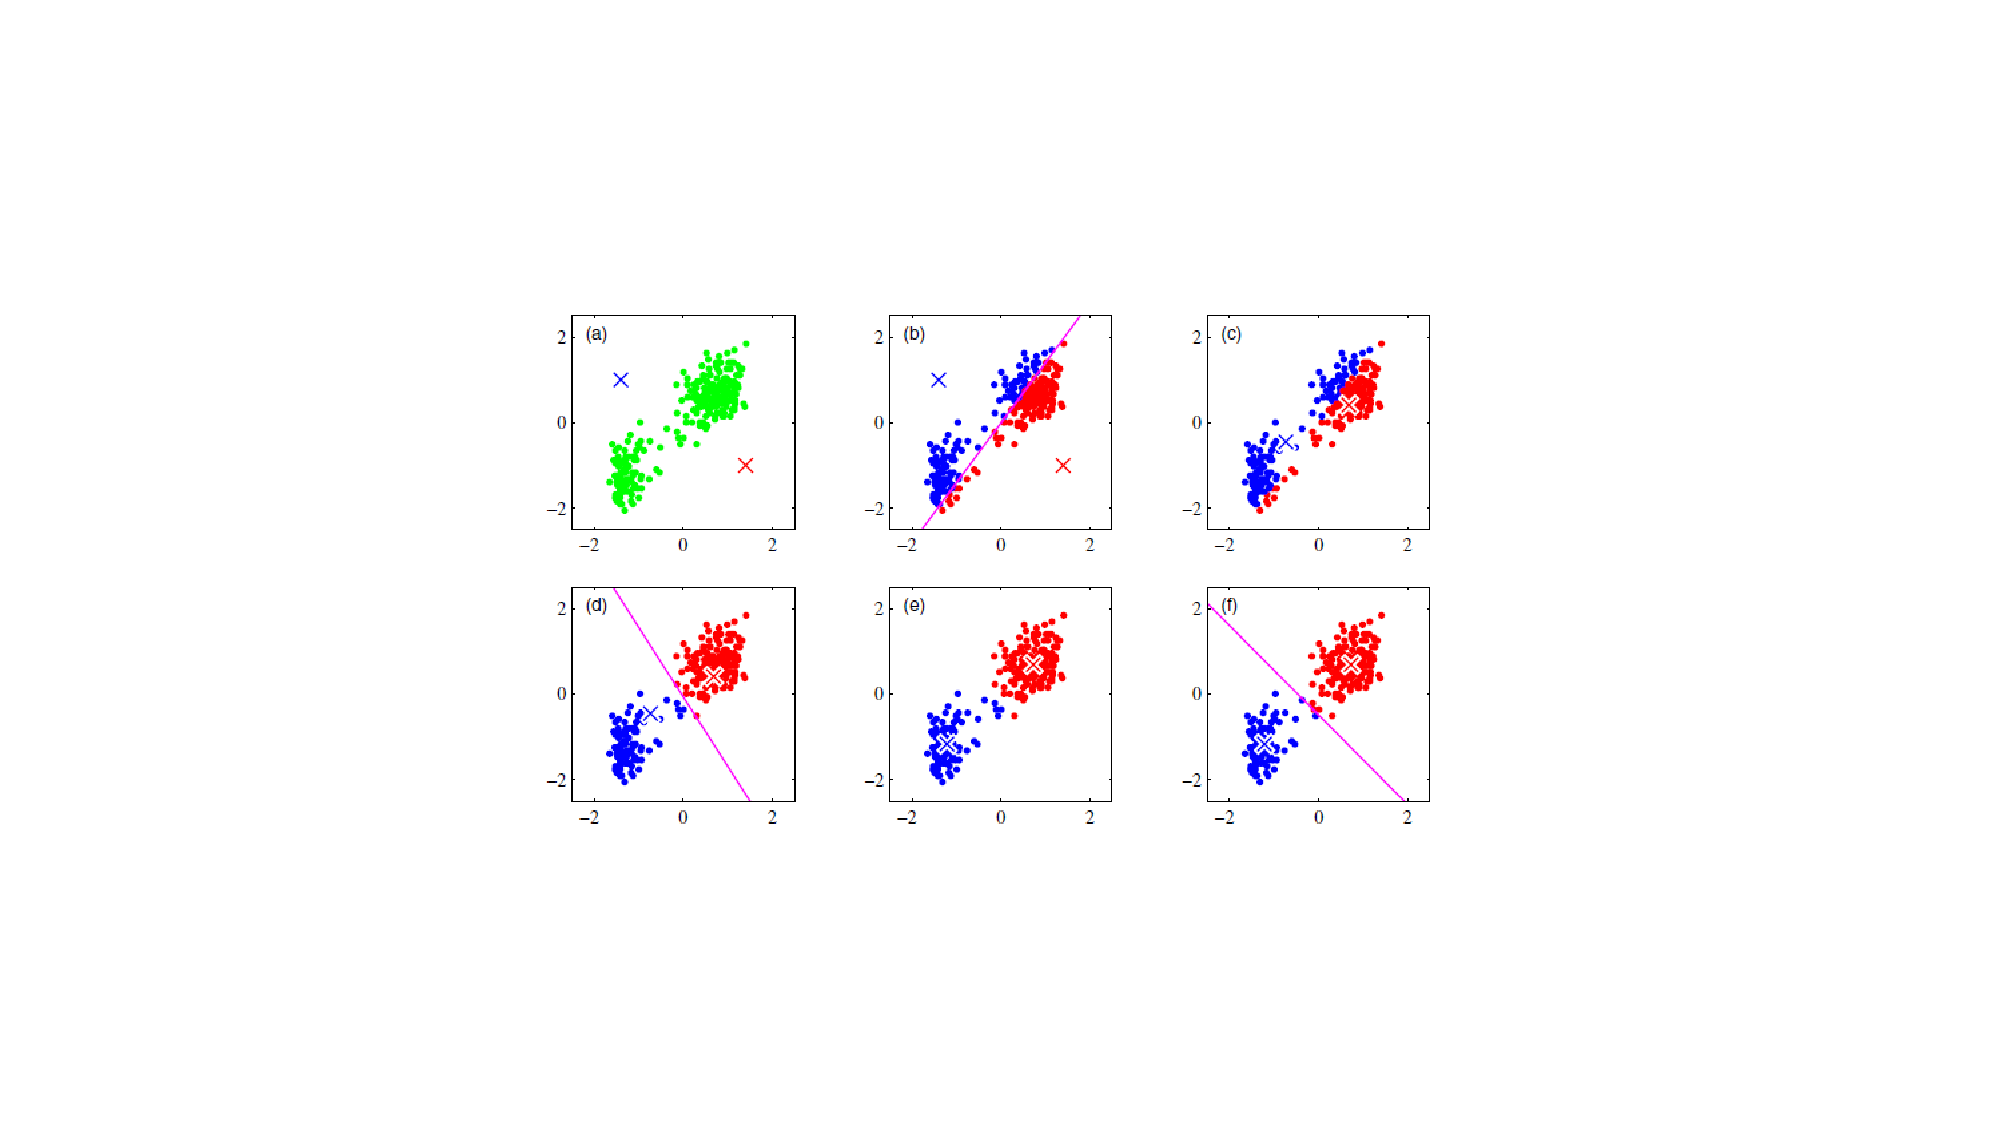
\includegraphics[trim=2.8in 2in 2in 1.8in,width=1.2\textwidth,clip]{../figures/kmeansstages.pdf}
  
\end{titledslide}
%%%%%%%%%%%%%%%%%%%%%%%%%%%%%%%%%%%%%%%%%%%%%%%%%%%%%%%%%%%%%%%%%%%%%%
\begin{titledslide}{$k$-means optimisation}

  \begin{itemize}
  \item $r_{nk} = 1$ if datapoint $\xvec_{n}$ is assigned to cluster $k$.
  \item $\bmu_{k}$ is the mean of cluster $k$.
  \end{itemize}
  
  \begin{equation}
    \label{eq:rnk}
    r_{nk} =
    \begin{cases}
      1 & \mbox{if $k= \arg\min_{j} ||\xvec_{n} - \bmu_{j}||^{2}$} \\
      0 & \mbox{otherwise} \\
    \end{cases}
  \end{equation}

  \begin{equation}
    \label{eq:mean}
    \bmu_{k} = \frac{\sum_{n} r_{nk}\xvec_{n}}{\sum_{n} r_{nk}}
  \end{equation}
  
\end{titledslide}
%%%%%%%%%%%%%%%%%%%%%%%%%%%%%%%%%%%%%%%%%%%%%%%%%%%%%%%%%%%%%%%%%%%%%%
\begin{titledslide}{Gaussian mixture distribution}


  Well, here it is \cite[\S 9.2]{bishop06:_patter_recog_machin_learn}

  \begin{equation}
    \label{eq:guassmix}
    p(\xvec) = \sum_{k=1}^{K} \pi_{k} \gauss(\xvec|\bmu_{k},\bcov_{k})
  \end{equation}

  We can associate the \emph{mixing coefficients} $\pi_k$ with a $K$-dimensional
  random variable \xvec{} where:
  \begin{eqnarray*}
    \label{eq:zk}
    z_{k} & \in & \{0,1\} \\
    \sum_{k} z_{k} &= & 1 \\
    p(z_{k}=1)  & = & \pi_{k} \\
  \end{eqnarray*}
  so we have
  \begin{equation}
    \label{eq:guassmixtwo}
    p(\xvec) = \sum_{\zvec} p(\zvec) p(\xvec|\zvec) = \sum_{k=1}^{K} \pi_{k} \gauss(\xvec|\bmu_{k},\bcov_{k})
  \end{equation}

  
\end{titledslide}
%%%%%%%%%%%%%%%%%%%%%%%%%%%%%%%%%%%%%%%%%%%%%%%%%%%%%%%%%%%%%%%%%%%%%% 
\begin{titledslide}{Responsibility and sampling}

  \begin{itemize}
  \item Now we have a full joint distribution $p(\xvec,\zvec)$ we can
    define the \emph{responsibility} that component $k$ has for
    `explaining' observation \xvec
  \end{itemize}
  \begin{equation}
    \label{eq:responsibility}
    \gamma(z_{k}) = p(z_{k}=1|\xvec)
  \end{equation}

  \begin{itemize}
  \item To sample from a Gaussian mixture just use ancestral sampling:
    sample from $p(\zvec)$, and then from $p(\xvec|\zvec)$. 
  \end{itemize}
  
\end{titledslide}
%%%%%%%%%%%%%%%%%%%%%%%%%%%%%%%%%%%%%%%%%%%%%%%%%%%%%%%%%%%%%%%%%%%%%%
\begin{titledslide}{Soft clustering with Gaussian mixtures}

  \vskip1cm

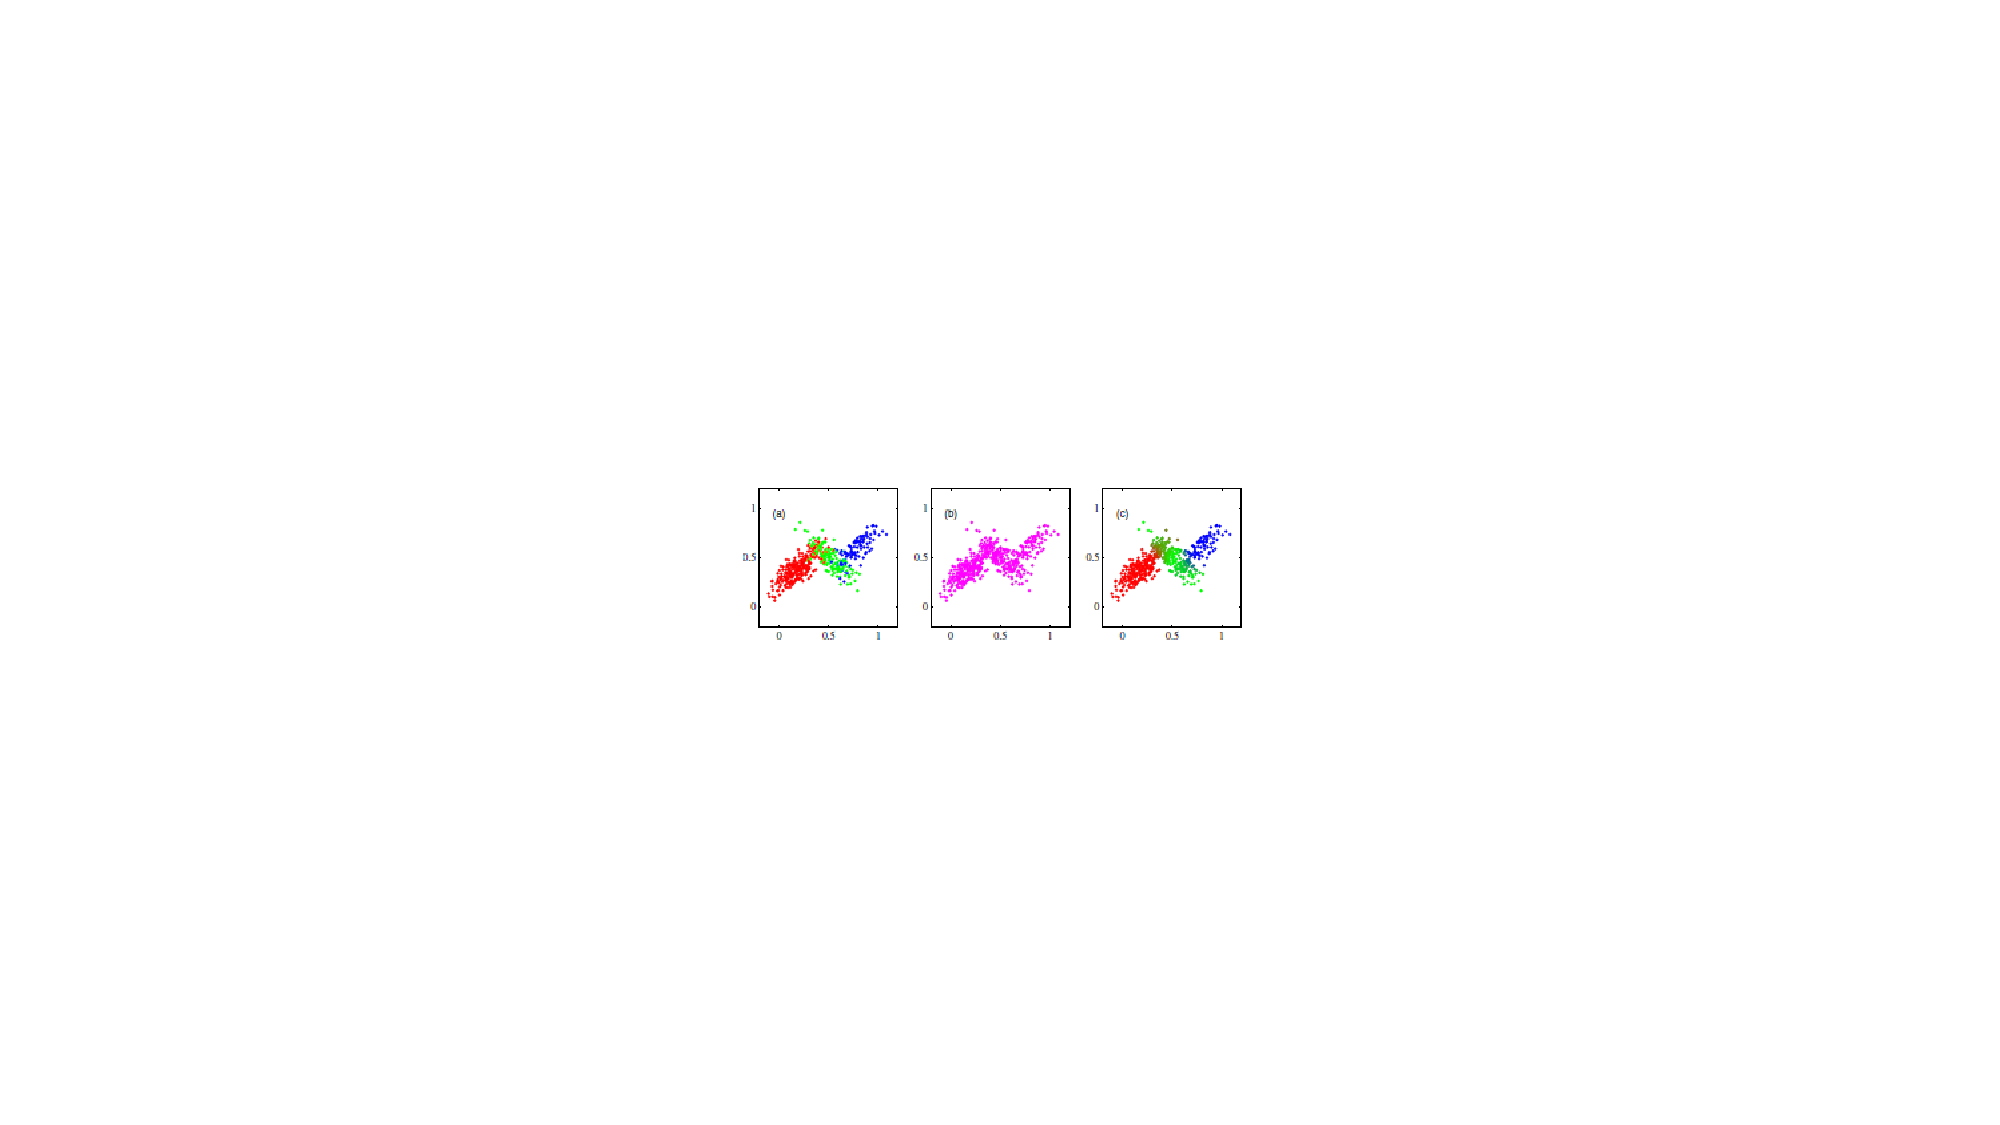
\includegraphics[trim=4.8in 2in 2in 2.8in,width=1.8\textwidth,clip]{../figures/gmplots.pdf}

  
\end{titledslide}
%%%%%%%%%%%%%%%%%%%%%%%%%%%%%%%%%%%%%%%%%%%%%%%%%%%%%%%%%%%%%%%%%%%%%%
\begin{titledslide}{More clustering with Gaussian mixtures}

  \begin{itemize}
  \item If we want we can put restrictions on the covariance matrices
    of the Gaussians in the mixture.
  \item Let's have a look at \cite[p.729]{pml1Book}
  \end{itemize}
  
\end{titledslide}
%%%%%%%%%%%%%%%%%%%%%%%%%%%%%%%%%%%%%%%%%%%%%%%%%%%%%%%%%%%%%%%%%%%%%%
\begin{titledslide}{(Soft) clustering by MLE of a Gaussian mixture}

  \begin{itemize}
  \item Given data \Xvec{} (and a fixed number $K$ of component Gaussians) we 
    can use MLE to get a particular Gaussian mixture distribution.
  \item This gives us a `soft clustering'.
  \item Here's the log-likelihood
    \cite[433]{bishop06:_patter_recog_machin_learn}:
  \end{itemize}
  \begin{equation}
    \label{eq:loglik}
    \ln p(\Xvec|{\bm \pi}, \bmu, {\bm \Sigma}) = \sum_{n=1}^{N} \ln
     \left\{ \sum_{k=1}^{K} \pi_{k} \gauss(\xvec_{n}|\bmu_{k},{\bm \Sigma}_{k}) \right\}  
  \end{equation}

  \begin{itemize}
  \item Number of problems:
    \begin{enumerate}
    \item Possible singularities
    \item Symmetry/nonidentifiability
    \item No closed form for the MLE
    \end{enumerate}
  \item Queue the EM algorithm \dots
  \end{itemize}
  
\end{titledslide}

%%%%%%%%%%%%%%%%%%%%%%%%%%%%%%%%%%%%%%%%%%%%%%%%%%%%%%%%%%%%%%%%%%%%%%
\begin{titledslide}{Reading}

  \begin{itemize}
  \item Bishop \S9.1 (you can skip \S9.1.1 but it's an interesting
    read).
  \item Bishop \S9.2 up to \S9.2.1
  \item Murphy \S21.3 up to \S21.3.3
  \end{itemize}
  
  
\end{titledslide}
%%%%%%%%%%%%%%%%%%%%%%%%%%%%%%%%%%%%%%%%%%%%%%%%%%%%%%%%%%%%%%%%%%%%%%
\begin{titledslide}{Problems and quizzes}

  \begin{itemize}
  \item Bishop Exercise 9.1
  \item Bishop Exercise 9.3
  \item Quizzes:
    \begin{itemize}
    \item Week~5: k-means and Mixtures of Gaussians
    \end{itemize}
  \end{itemize}
  
\end{titledslide}
%%%%%%%%%%%%%%%%%%%%%%%%%%%%%%%%%%%%%%%%%%%%%%%%%%%%%%%%%%%%%%%%%%%%%%
\bibliographystyle{alpha}
\bibliography{../ml}

\end{document}
%%%%%%%%%%%%%%%%%%%%%%%%%%%%%%%%%%%%%%%%%%%%%%%%%%%%%%%%%%%%%%%%%%%%%% 
